\newif\ifJPN
\JPNtrue % 日本語モード
\JPNfalse % 英語モード

\ifJPN
\documentclass{bxjsarticle}
\else
\documentclass[english]{bxjsarticle}
\fi
\usepackage{fontspec}
\setsansfont{Noto Sans CJK JP}
\setmainfont{Noto Serif CJK JP} % xelatexで日本語対応
\usepackage{tikz}
\usetikzlibrary{shapes.geometric, arrows.meta, positioning, fit, backgrounds}
\usepackage{hyperref}

%\usepackage{geometry}
%\geometry{a4paper, margin=25mm}

\ifJPN
  \title{私のプロジェクト全体図}
  \author{山元 啓史\\東京科学大学}
\else
  \title{Overview of My Projects}
  \author{Hilofumi Yamamoto\\Institute of Science Tokyo}
\fi
\date{\today} % 改行記号を削除

\renewcommand{\arraystretch}{1.4}
\newcommand{\customsmall}{\fontsize{9pt}{9pt}\selectfont}
\begin{document}

\maketitle

\begin{abstract}
\ifJPN
この文書は、私が関わっているすべてのプロジェクトを体系的に整理し、プロセス文法モデルを中心とした研究・教育・技術基盤の関係性を図示したものである。
プロジェクトは、古典文学の翻訳や教育実践、技術基盤の整備など多岐にわたり、それぞれが相互に関連し合いながら進行している。
\else
This document systematically organizes all the projects I am involved in, illustrating the relationships between research, education, and technical infrastructure centered around the Process Grammar Model.
The projects cover a wide range of areas, including the translation of classical literature, educational practices, and the establishment of technical infrastructure, all of which are progress in mutual relation.
\fi
\end{abstract}

\ifJPN
\section{プロセス文法モデル(PGM)}
\else
  \section{Process Grammar Model (PGM)}
\fi

\begin{itemize}
\ifJPN
  \item 即時文法(Immediate Grammar)と調整文法(Adjustive Grammar)に基づく理論。
  \item Kahnemanの二重過程理論の影響を受けつつ、人間の自然な言語使用を分析する。
  \item 喚体句、感動詞、相づちなどの"瞬間のことば"にも規則性があることを記述。
\else
  \item Theory based on Immediate Grammar and Adjustive Grammar.
  \item Influenced by Kahneman's dual-process theory, analyzing natural language use in humans.
  \item Describing the regularity of "instant words" such as exclamatory phrases, interjections, and backchannels.
\fi
\end{itemize}

\ifJPN
\section{古典研究プロジェクト}
\else
  \section{Classical Literature Research Projects}
\fi
\begin{itemize}
\ifJPN
  \item 『伊勢物語』翻訳・注釈:逐語訳と自然訳の併記、語りと即時性の研究。
  \item 『土佐日記』翻訳・注釈:語り手のユーモアと現在性を分析。
  \item JSON形式による注釈・訳語記録の構造化。
\else
  \item Translation and annotation of "Ise Monogatari": Bilingual translation and research on narrative and immediacy.
  \item Translation and annotation of "Tosa Nikki": Analysis of the narrator's humor and present-oriented viewpoint.
  \item Structuring annotations and translations in JSON format.
\fi
\end{itemize}

\ifJPN
\section{教育プロジェクト}
\else
  \section{Educational Projects}
\fi

\begin{itemize}
\ifJPN
  \item \textbf{D4E}: Dictation for Every Day(2020年〜)
  \begin{itemize}
    \item 約150エピソード作成済み、現在改訂中。
    \item Markdown/HTML対応テキスト化構想あり。
  \end{itemize}
  \item \textbf{AEAD}: An Expression A Day(2024年〜)
  \begin{itemize}
    \item 即時文法の辞書化を目指した1日1表現の記録。
    \item JSON構造に"tags-ja/en"や"adjusted-expression"を記録。
  \end{itemize}
\else
  \item \textbf{D4E}: Dictation for Every Day (2020 - present)
  \begin{itemize}
    \item Approximately 150 episodes created, currently under revision.
    \item Plans for text conversion compatible with Markdown/HTML.
  \end{itemize}
  \item \textbf{AEAD}: An Expression A Day (2024 - present)
  \begin{itemize}
    \item Recording of one expression a day aimed at creating a dictionary of immediate grammar.
    \item Recording "tags-ja/en" and "adjusted-expression" in JSON structure.
  \end{itemize}
\fi
\end{itemize}

\ifJPN
\section{技術基盤}
\else
\section{Technical Infrastructure}
\fi

\begin{itemize}
\ifJPN
  \item GitHub: 毎日アップロード、Zenodoで公開・アクセス分析。
  \item LaTeX + JSON によるドキュメント整備。
  \item sed, jq, awk による軽量処理優先。
\else
  \item GitHub: Daily uploads, public access analysis via Zenodo.
  \item Document maintenance using LaTeX + JSON.
  \item Lightweight processing prioritized with sed, jq, awk.
\fi
\end{itemize}

\ifJPN
\section{全体構成図}
\else
  \section{Overall Structure Diagram}
\fi

\begin{center}
  \scalebox{0.8}{
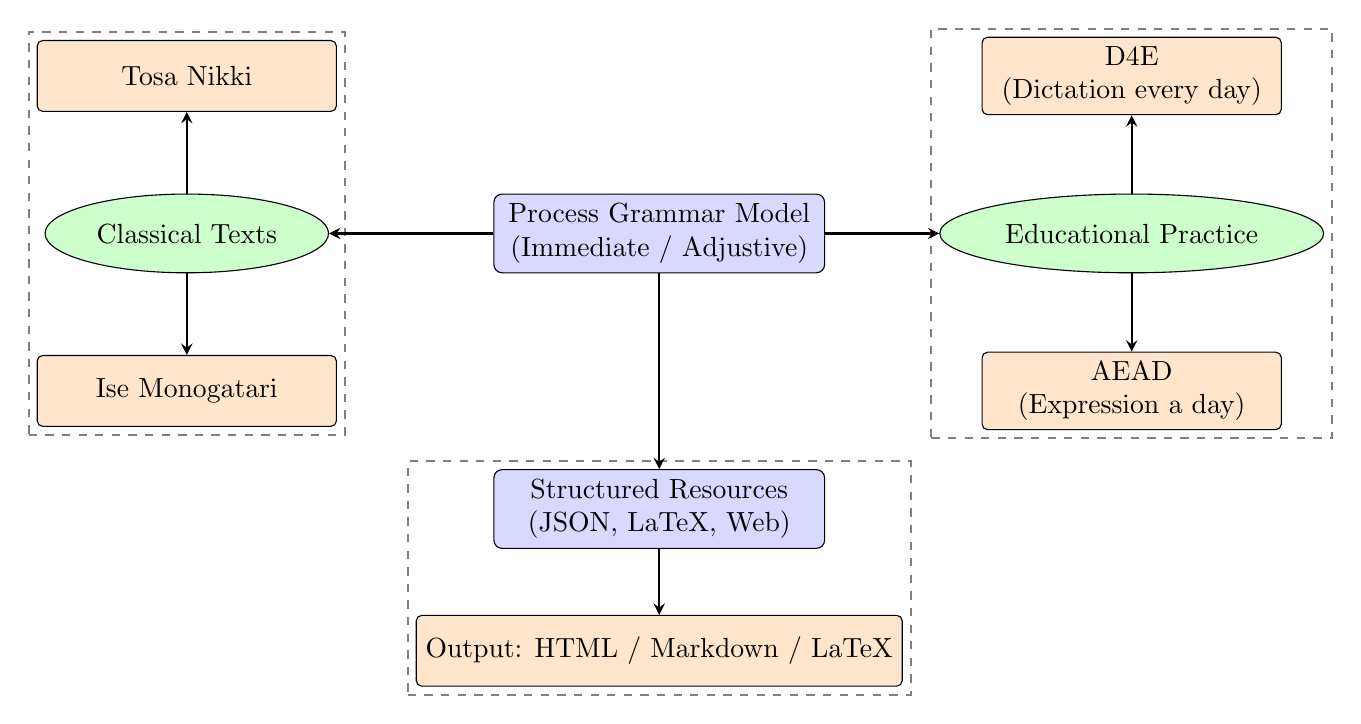
\begin{tikzpicture}[node distance=.5cm and 1.2cm]
  \tikzstyle{mainnode} = [rectangle, rounded corners=3pt, minimum width=4.2cm, minimum height=1cm, align=center, draw=black, fill=blue!15]
  \tikzstyle{category} = [ellipse, minimum width=3.6cm, minimum height=1cm, align=center, draw=black, fill=green!20]
  \tikzstyle{subnode} = [rectangle, rounded corners=2pt, minimum width=3.8cm, minimum height=0.9cm, align=center, draw=black, fill=orange!20]
  \tikzstyle{connector} = [thick,->,>=stealth]

  % Central node
  \node (pgm) at (0,0) [mainnode] {Process Grammar Model\\(Immediate / Adjustive)};

  % Left side: Classical texts
  \node (classical) at (-6,0) [category] {Classical Texts};
  \node (tosa) at (-6,2) [subnode] {Tosa Nikki};
  \node (ise) at (-6,-2) [subnode] {Ise Monogatari};

  % Right side: Educational practice
  \node (education) at (6,0) [category] {Educational Practice};
  \node (d4e) at (6,2) [subnode] {D4E\\(Dictation every day)};
  \node (aead) at (6,-2) [subnode] {AEAD\\(Expression a day)};

  % Bottom side: Infrastructure
  \node (infra) at (0,-3.5) [mainnode] {Structured Resources\\(JSON, LaTeX, Web)};
  \node (output) at (0,-5.3) [subnode] {Output: HTML / Markdown / LaTeX};

  % Arrows
  \draw[connector] (pgm) -- (classical);
  \draw[connector] (pgm) -- (education);
  \draw[connector] (pgm) -- (infra);
  \draw[connector] (classical) -- (tosa);
  \draw[connector] (classical) -- (ise);
  \draw[connector] (education) -- (d4e);
  \draw[connector] (education) -- (aead);
  \draw[connector] (infra) -- (output);

  % Background groups
  \begin{pgfonlayer}{background}
    \node[draw=gray, dashed, thick, inner sep=0.1cm, fit=(tosa)(ise)(classical)] {};
    \node[draw=gray, dashed, thick, inner sep=0.1cm, fit=(d4e)(aead)(education)] {};
    \node[draw=gray, dashed, thick, inner sep=0.1cm, fit=(infra)(output)] {};
  \end{pgfonlayer}
\end{tikzpicture}
}
\end{center}

\ifJPN
\section{プロジェクト一覧表}
\else
  \section{Project List}
\fi

\ifJPN
\begin{table}[ht]\centering
\caption{プロジェクト一覧}
\customsmall
\scalebox{0.8}{
\begin{tabular}{lllll}\noalign{\hrule height .8pt}
\hline
\textbf{プロジェクト} &\textbf{略称}& \textbf{主な対象} & \textbf{目的} & \textbf{共通する軸} \\
\hline
プロセス文法モデル& PGM & 人間の発話過程 & 即時性 vs 調整性の記述 & 文法の「動的モデル」化 \\
土佐日記翻訳 & TOSA & 古典日本文学 & 現代語・英語へ逐次訳と意訳 & 語りの即時性、翻訳の構造化 \\
伊勢物語翻訳 & ISE &  短歌・物語の交差 & 文体・空間表現・視点の構造分析 & 美的形式の即時性と構造的連鎖 \\
Dictation for Every Day &D4E & 現代日本語会話 & 音声と言語反応の実践練習 & 即時的な発話パターンの実例集 \\
An Expression A Day&AEAD & 口語的日本語表現 & 即時文法の収集・タグ付け & 日常に根ざした即時反応の体系化 \\
\end{tabular}}
\end{table}
\else
  \begin{table}[ht]\centering
    \caption{Project List}
    \customsmall
    \renewcommand{\arraystretch}{1.2}
    \scalebox{1.0}{
      \begin{tabular}{llp{90mm}}\noalign{\hrule height .8pt}
        \hline
        \textbf{Project} &\textbf{Abbr.}& \textbf{Main Target}/\textbf{Purpose}/\textbf{Common Axis} \\
        \hline
        Process Grammar Model& PGM & Human Speech Process / Description of Immediacy vs Adjustiveness / Dynamic Modeling of Grammar \\
        Tosa Nikki Translation & TOSA & Classical Japanese Literature / Sequential and free translation into modern Japanese and English / Immediacy of Narrative, Structuring of Translation \\
        Ise Monogatari Translation & ISE & Intersection of Tanka and Narrative / Structural Analysis of Style, Spatial Expression, and Perspective / Immediacy of Aesthetic Form and Structural Chain \\
        Dictation for Every Day &D4E & Modern Japanese Conversation / Practical Practice of Voice and Language Response / Collection of Immediate Speech Patterns \\
        An Expression A Day&AEAD & Colloquial Japanese Expressions / Collection and Tagging of Immediate Grammar / Systematization of Immediate Response Rooted in Daily Life \\
      \end{tabular}}
    \end{table}
  \fi

\end{document}
